\def\allfiles{}
\documentclass{package/fancy-book}
\setlength{\parindent}{2em}
\usepackage[UTF8]{ctex}
%%%%%%%%%% Default Package %%%%%%%%%%%%%
\usepackage{package/color-env}
\usepackage{package/quiver}
\usepackage{background}
\usepackage[object=vectorian]{pgfornament} %% used in title.tex
\usepackage{calligra} %%% (optional) to make the Title text beautiful 
\usepackage{lipsum}  %% for dummy text 
\usepackage{amssymb,amsmath,amsfonts}  %%% for maths
\usepackage{datetime}

%%%%%% Optional Packages %%%%%%%
\usepackage{lettrine} %% for nice looking 
\usepackage{GoudyIn} %% first Letter of the paragraph
\renewcommand{\LettrineFontHook}{\color{black}\GoudyInfamily{}}
\LettrineTextFont{\itshape}
\setcounter{DefaultLines}{3}%
%%%%%%%%%%%%%%%%%%%%%%%%%%%%%%%%%%%%%
\usepackage{datetime2}
\usepackage{fourier-orns}
\newcommand{\ornamento}{\vspace{2em}\noindent \textcolor{darkgray}{\hrulefill~ \raisebox{-2.5pt}[10pt][10pt]{\leafright \decofourleft 
\decothreeleft  \aldineright \decotwo \floweroneleft \decoone   \floweroneright 
\decotwo \aldineleft\decothreeright \decofourright \leafleft} ~  \hrulefill \\ \vspace{2em}}}

% 命令
\newcommand{\id}{\mathrm{id}}
\newcommand{\Hom}{\mathrm{Hom}}
\newcommand{\Ext}{\mathrm{Ext}}
\newcommand{\Tor}{\mathrm{Tor}}
\newcommand{\N}{\mathbb{N}}
\newcommand{\Z}{\mathbb{Z}}
\newcommand{\Q}{\mathbb{Q}}
\newcommand{\R}{\mathbb{R}}
\newcommand{\C}{\mathbb{C}}
\newcommand{\HH}{\mathbb{H}}
\newcommand{\RP}{\mathbb{RP}}
\newcommand{\cC}{\mathcal{C}}

%%%% Bibliography %%%%%%%%%
% Required packages are included in notes class
% Can be tweaked in the notes.cls file itself
\addbibresource{resource/references.bib}
\includeonly{title,tex/2.tex}
\begin{document}
\begin{titlepage}

%%%%%%%%%%%%%%%%%%%%%%%%%%%%%%%%%%%% Inspired From  %%%%%%%%%%%%%%%%%%%%%%%%%%%%%%%%%%%%%%%%%%%%%%%%% 
%%%%  https://www.reddit.com/r/LaTeX/comments/j9d739/hello_world_in_latex_is_a_lot_cooler/   %%%%%
%%%%%%%%%%%%%%%% If this doesn't look nice then you may remove it %%%%%%%%%%%%%%%%%%%%%%%%%%

\backgroundsetup{
scale=1,
opacity=1,
angle=0,
color=black,
contents={
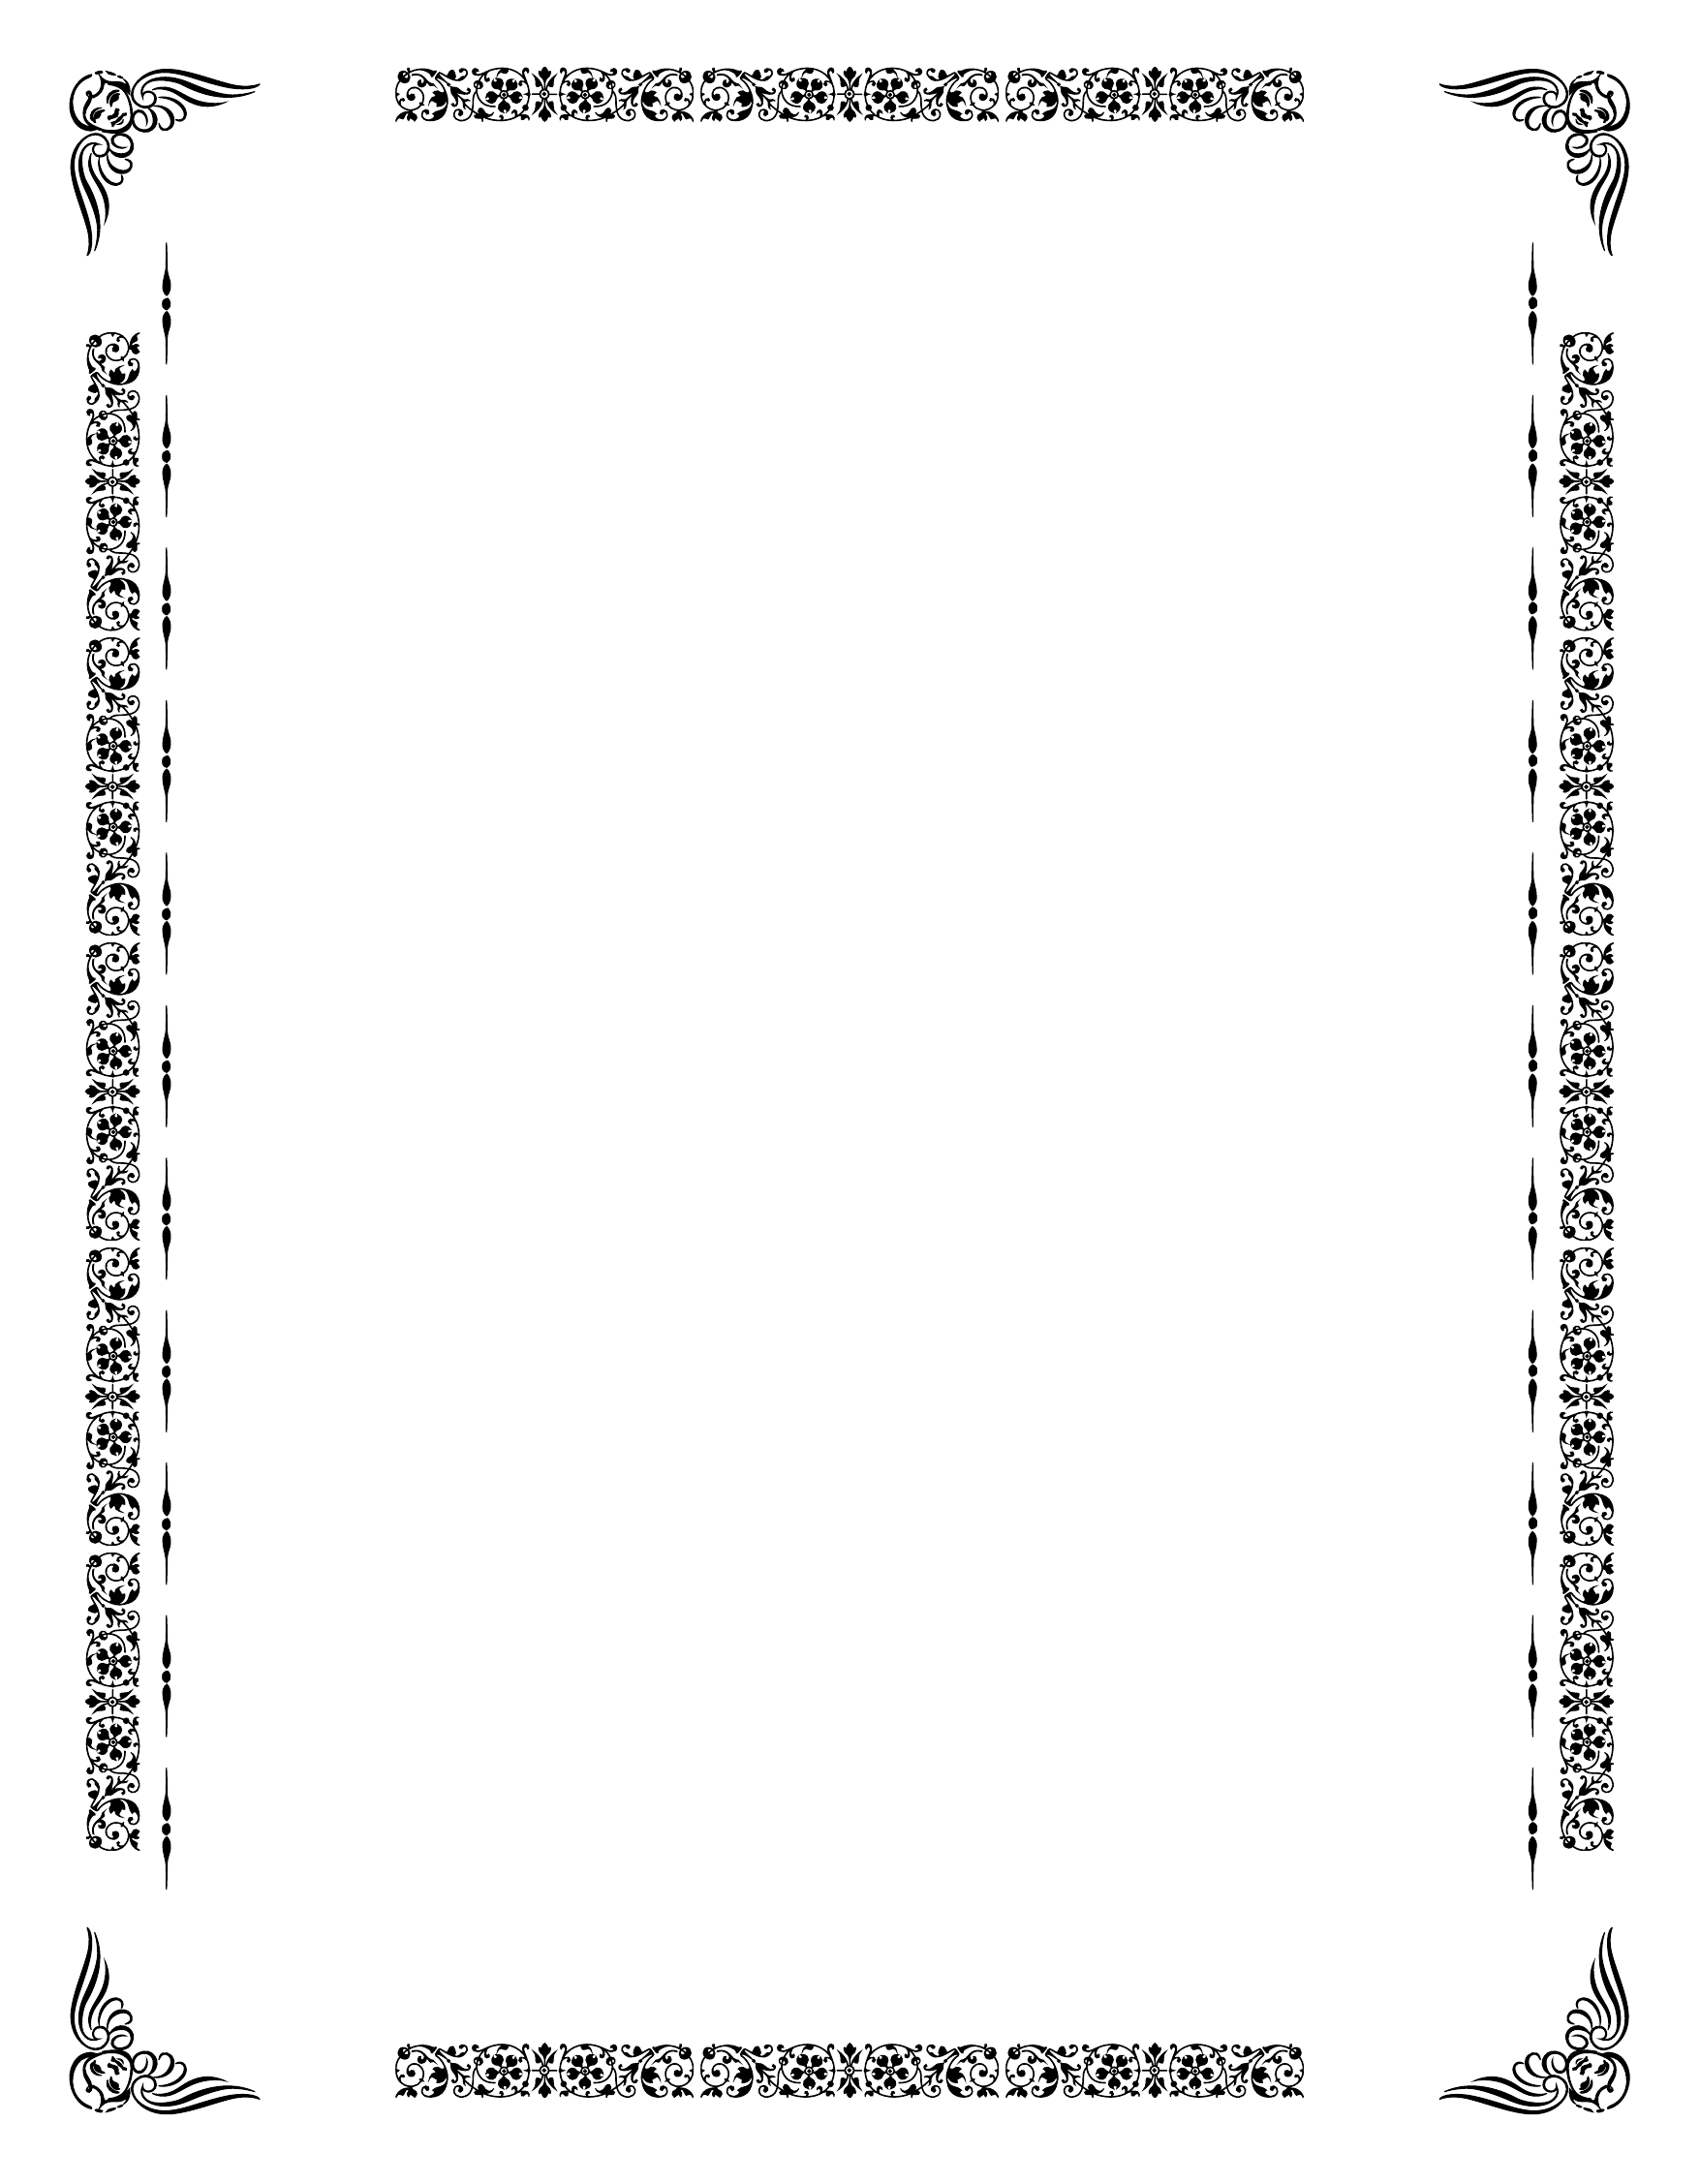
\begin{tikzpicture}[color=black, every node/.style={inner sep= 15pt}]
\node (NW) [anchor=north west] at (current page.north west){\pgfornament[width=2.5cm] {131}};
\node (NE) [anchor=north east] at (current page.north east){\pgfornament[width=2.5cm, symmetry=v]{131}};
\node (SW) [anchor=south west] at (current page.south west){\pgfornament[width=2.5cm, symmetry=h]{131}};
\node (SE) [anchor=south east] at (current page.south east){\pgfornament[width=2.5cm, symmetry=c]{131}};
\foreach \i in {-4,0,4}
\node[anchor=north,xshift=\i cm] at (current page.north){\pgfornament[scale=0.25,symmetry=v]{71}};
\foreach \i in {-4,0,4}
\node[xshift=\i cm, yshift=32.25 pt] at (current page.south){\pgfornament[scale=0.25,symmetry=v]{71}};
\foreach \i in {-8,-4,0,4,8}
\node[yshift=\i cm, xshift=32.25pt, rotate=90] at (current page.west){\pgfornament[scale=0.25,symmetry=v]{71}};
\foreach \i in {-8,-4,0,4,8}
\node[yshift=\i cm, xshift=-32.25pt, rotate=90] at (current page.east){\pgfornament[scale=0.25,symmetry=v]{71}};
\foreach \i in {-11,-9,...,7,9}
\node[anchor=west, yshift=\i cm, xshift=52.25pt, rotate=90] at (current page.west){\pgfornament[scale=0.1]{80}};
\foreach \i in {-11,-9,...,7,9}
\node[anchor=east, yshift=\i cm, xshift=-52.25pt, rotate=-90] at (current page.east){\pgfornament[scale=0.1]{80}};
\end{tikzpicture}
}}

%%%%%%%%%%%%%%%%%%%%%%%%%%%%%%%%%%%%%%%%%%%%%%%%%%%%%%%%%%%%%%%%%%%%%%%%%%%%%%%%%%%%%%%%%%%%%%%%%%%%%%%%%%%%%%%%%%

\centering % Centre everything on the title page
		
\scshape % Use small caps for all text on the title page

\vspace*{\baselineskip} % White space at the top of the page

%------------------------------------------------
%	Title
%------------------------------------------------

\rule{\textwidth}{1.6pt}\vspace*{-\baselineskip}\vspace*{2pt} % Thick horizontal rule
\rule{\textwidth}{0.4pt} % Thin horizontal rule

\vspace{0.75\baselineskip} % Whitespace above the title

{\huge \calligra{\textbf{Note for Homological Algebra} }\\} % Title

\vspace{0.75\baselineskip} % Whitespace below the title

\rule{\textwidth}{0.4pt}\vspace*{-\baselineskip}\vspace{3.2pt} % Thin horizontal rule
\rule{\textwidth}{1.6pt} % Thick horizontal rule

\vspace{2\baselineskip} % Whitespace after the title block

%------------------------------------------------
%	Subtitle
%------------------------------------------------

\Huge{范畴论笔记} 

\vspace*{3\baselineskip} % Whitespace under the subtitle



\vspace{0.5\baselineskip} 

{\scshape   \LARGE Edited by\\  颜成子游/南郭子綦} % Editor list
\vspace{0.2\baselineskip} 


\vfill 
\Large{最后一次编译时间:\DTMnow}
%------------------------------------------------
% Author
%------------------------------------------------

\begin{figure}[!h]
    \centering
    
\includegraphics[width = 3cm, height= 3cm]{resource/icon.png}%% include the university icon here
\end{figure}
\vspace{0.3\baselineskip} 

\end{titlepage}
\backgroundsetup{contents={}} %% to remove background and watermark from other pages
\tableofcontents

\quad

范畴论基础是学习现代数学理论重要的语言。很多时候如果预先学习过范畴论,就可以很好的了解许多已知的数学理论。我们将会以李文威所著的《代数学方法》为讲义,攥写该笔记。以此在将来遇到该门语言时可以进行快速的复习。

由于范畴本身的概念在攥写笔记中可以得到反复强化,因此我们省略范畴论中最最基础的定义,直接从函子范畴开始攥写笔记。
\chapter{流形上的非退化光滑函数}
\section{Morse函数}
我们先用一个引理说明在非临界点$M$的平凡性质。
\begin{lemma}[非临界点]
	设$M^a=\{p\in M|f(p)\leq a\}$。若$a$不是临界值,则$M^a$是带边的光滑流形。
\end{lemma}

引理的证明留作练习。主要使用到隐函数定理以及带边流形的定义。

\begin{definition}[非退化点]
	考虑$M$上的函数$f$.若在$f$的临界点$p$处存在一个局部坐标$(U;x^i)$使得矩阵:
	\begin{align}\label{Hess}
		(\frac{\partial^2 f}{\partial x^i\partial x^j}(p))
	\end{align}
	非奇异,则称$p$是一个非退化点。
\end{definition}
这里需要注意的是,$p$的非退化性显然与局部坐标$x^i$无关。因此$p$的非退化性是$f$内蕴的性质。

如果$p$是$f$的临界点,我们就可以定义在$T_pM$上的双线性函数$f_{**}$。若$v,w \in T_pM$,用$\tilde{v}$和$\tilde{w}$表示在$p$处值为$v,w$的向量场。定义:
\begin{align}
	f_{**}(v,w)=\tilde{v}_p(\tilde{w}f)
\end{align}

我们断言:
\begin{lemma}
	$f_**$是对称的良定双线性函数。
\end{lemma}
\begin{proof}
	考虑:
	\begin{align}
		\tilde{v}_p(\tilde{w}f)-\tilde{w}_p(\tilde{v}f)=[\tilde{v},\tilde{w}]_p(f)=0
	\end{align}
	最后一个等号成立,是因为$p$是$f$的临界点。

	从而$f_{**}$是对称的。因此,$\tilde{v}_p(\tilde{w}f)$与$\tilde{v}$的选取无关,$\tilde{w}_p(\tilde{v}f)$与$\tilde{w}$的选取无关.

	于是$f_{**}$与$\tilde{v},\tilde{w}$的选取都无关,因而是良定的双线性函数。
\end{proof}
\begin{definition}[Hessian,指数,零化度]
    \quad \quad 称$f_{**}$为函数$f$在$p$处的Hessian双线性函数。
	
	而$f_{**}$的指数定义为满足$f_**$限制在上为负定双线性函数的子空间$V$的最大维数。$f_{**}$的零化度定义为$f_{**}$的零空间$W$的维数,即子空间$W=\{v \in V|f_{**}(v,w)=0,\forall w\in V\}$的维数。
\end{definition}

可以验算$f_{**}$在坐标$(U;x^i)$下给出的就是矩阵\ref{Hess}.显然,$f$在$p$处非退化等价于$f_{**}$的零化度是$0$。$f_{**}$的指数也称为$f$在$p$处的指数。

\begin{lemma}[Morse引理]\label{Morse-lemma}
	设$p$是$f$的非退化点,则存在一个$p$处的局部坐标$(U;y^i)$满足$y^i(p)=0,\forall i$且:
	\begin{align}
		f(q)=f(p)-(y^1)^2-\dots-(y^\lambda)^2+(y^{\lambda+1})^2+\dots+(y^n)^2
	\end{align}
	在整个$U$上都成立.其中$\lambda$是$f$在$p$处的指数。
\end{lemma}
\begin{proof}
	我们首先说明如果$f$拥有这样的表达式,则指数为$\lambda$.

	对于坐标$(z^i)$,若:
	\begin{align*}
		f(q)=f(p)-(z^1(q))^2-\dots-(z^\lambda(q))^2+\dots+(z^n(q))^2
	\end{align*}
	则容易求出$f_{**}$在该坐标下的矩阵为$\mathrm{diag}(-2,\dots,-2,2,\dots,2)$.其中$-2$一共有$\lambda$个。

	因此存在一个$\lambda$维的子空间使得$f_{**}$是负定的,存在一个$n-\lambda$维的子空间$V$使得$f_{**}$是正定的。如果$p$处的指数大于$\lambda$,则对应的子空间与$V$相交不为空。但这是不可能的,因此$\lambda$是$f$在$p$处的指数。

	接下来我们说明$(y^i)$坐标存在。不妨设$p$是$\R^n$的原点且$f(p)=f(0)=0$.从而有:
	\begin{align}
		f(x_1,\dots,x_n)=\int_0^1\frac{\dd f(tx_1,\dots,x_n)}{\dd   t}\dd t=\int_0^1 \sum_{i=1}^n \pa{f}{x_i}(tx_1,\dots,tx_n)x_i\dd t
	\end{align}
	令$g_j=\int_0^1\pa{f}{x_i}(tx_1,\dots,tx_n)\dd t$,则$f=\sum_j  x_jg_j$在$0$处的一个邻域上成立。

	因为$0$是$f$的临界点,从而$\pa{f}{x)i}(0)=0$。这意味着$g_j(0)=\pa{f}{x_i}(0)$.因而对$g_j$作上述$f$同样的分解:
	\begin{align*}
		f(x_1,\dots,x_n)=\sum_{i,j} x_ix_jh_{ij}(x_1,\dots,x_n)
	\end{align*}
	
	不妨假设$h_{ij}$关于$i,j$对称。通过计算,不难验证矩阵$(h_{ij}(0))$等于:
	\begin{align*}
		(\frac{1}{2}\frac{\partial^2f}{\partial x^i\partial x^j}(0))
	\end{align*}
	因此$h_{ij}(0)$是非奇异的矩阵。仿照模仿有理标准型的构造,可以证明存在一组坐标$(y^i)$使得$f$呈现为引理中的形式。具体的构造办法详见Milnor原书。(附录)
\end{proof}

Morse引理的好处在于我们可以用指数唯一确定$f$在$p$处的一个标准形式。根据这个引理,可以得知$f$在非退化点$p$的一个邻域内只有$p$一个临界点。
\begin{corollary}
	非退化临界点是离散的。特别的,紧致流形$M$上的非退化临界点只有有限个。
\end{corollary}

\begin{definition}[Morse函数]
	若$f\in \mathcal{O}(M)$且只有非退化的临界点,则称该函数为Morse函数。
\end{definition}
Morse函数的好处是显而易见的。然而存在性则是一个问题。本节我们剩下的内容为下面的定理。
\begin{theorem}
	任何流形$M$上都存在一个可微的函数$f$,满足不存在退化临界点,且$M^a$对于任何$a \in \R$都是紧致的。
\end{theorem}

根据Whitney嵌入定理,任何流形都可以嵌入到维数足够高的欧氏空间。因而我们考虑$M$是$\R^n$的$k$维嵌入子流形(之后统称为“子流形”)。

定义$N \subset M\times \R^n$为:
\begin{align*}
	N=\{(q,v):q \in M,v\in T_q\R^n,v\perp M\}
\end{align*}
即$N$是$M$在$\R^n$中的法丛。不难验证$N$是$n$维的流形,且光滑的嵌入进$\R^{2n}$中。定义$E:N \to \R^n$为映射$(q,v)\mapsto q+v$.

\begin{definition}[焦点]
	称$e \in \R^n$是$(M,q)$重数为$\mu$的焦点,若$e=E(q,v),(q,v)\in N$且$E$在$(q,v)$处的Jacobian矩阵有零化度$\mu$.
\end{definition}

根据Sard定理,两个微分流形之间的可微映射的临界点是很有限的——临界值只有$0$测度。显然焦点是$E$的临界值,因而:
\begin{corollary}\label{0focus}
	对于几乎所有的$x \in \R^n$,$x$都不是$M$的焦点。
\end{corollary}

现在固定$p \in \R^n$.定义函数$f:M \to \R$为:
\begin{align}
	L_p=f:q\mapsto\|q-p\|^2
\end{align}
在坐标$(U;u^1,\dots,u^k)$下,$f$的表达式为:
\begin{align*}
	f(u^1,\dots,u^k)=\|\vec{x}(u^1,\dots,x^k)-\vec{p}\|^2=\vec{x}\vec{x}-2\vec{x}\vec{p}+\vec{p}\vec{p}
\end{align*}

因此可以计算:
\begin{align*}
	\pa{f}{u^i}=2\pa{\vec{x}}{u^i}\cdot(\vec{x}-\vec{p})
\end{align*}

因此$q$是$f$的临界点,当且仅当$q-p$垂直与$M$垂直。

考虑$f$的二阶导数。我们有:
\begin{align*}
	\frac{\partial^2 f}{\partial u^i\partial u^j}=2\pa{\vec{x}}{u^i}\pa{\vec{x}}{u^j}+\pa{\vec{x}}{u^i}u^j\cdot(\vec{x}-\vec{p})
\end{align*}

从而有
\begin{lemma}
	$q$是$f=L_p$的退化临界点等价于$p$是$(M,q)$的焦点。根据推论\ref{0focus},总存在这样的$L_p$使得该函数不存在退化的临界点。另外,若$q$是$L_p$的退化临界点,则该点的零化度是$p$的重数。
\end{lemma}

\section{临界值处的伦形}
\section{Morse不等式}


\chapter{Morse理论的应用——测地线变分}
\section{道路的能量积分}
\section{指标定理}
\section{道路空间的伦型}

\end{document}